% !TEX root = base.tex 

\chapter{Photochemical Reactivity of Bismuth Ferrite Ceramics}
\label{ch:bfo}


\chintro{The majority of the text in this chapter appears in \emph{ACS Applied Materials
\& Interfaces}, 2011, 3 (5), pp 1562-1567.\cite{Schultz:2011dl} It represents the
culmination of experimental work from the initial stages of Ph.D. research. The
interaction of visible light absorbing films on ferroelectric substrates provided the
initial research questions that lead to the research that makes up the bulk of this
document. It also represents further experiments regarding the effects of built-in
electric fields at the surface of ferroelectric semiconductors on photochemical
performance.}


\section{Background}
\label{sec:ch7background}


Spatially selective photochemical reactivity on the surfaces of ferroelectrics, initiated
by the absorption of \abbr{UV} light, has been used to make nanoscale patterns of reduced
metal.\cite{Giocondi:2001gz,Hanson:2006bq,Kalinin:2002iw,Tiwari:2009jv} The mechanism of
the spatially selective reactivity is thought to be the spontaneous polarization in the
ferroelectric domains, which bends the bands of electronic states so that photogenerated
electrons and holes are transported in opposite
directions.\cite{Anonymous:2011wc,FRIDKIN:1984tg} As a result, electrons are transported
to the surfaces of positive domains where reduction products form and holes are
transported to the surfaces of negative domains where oxidation products
form.\cite{Giocondi:2001gz,Burbure:2010go,Giocondi:2001bi,Burbure:2010ti,Bhardwaj:2010eh,Dunn:2007ja}

Spatially selective reactivity induced by ferroelectric polarization may also be
beneficial for water photolysis. The recombination of photogenerated charge carriers and
the back reaction of intermediate species are major factors that limit the efficiency of
water photolysis catalysts,\cite{Kudo:2008fk,Domen:1996um} and it is possible that these
processes will be mitigated by band bending in the domains. This concept has led to a
number of studies involving water
photolysis\cite{Inoue:2009bh,Inoue:1990vc,Anonymous:lTM5YSKy} and spatially selective
reactivity on ferroelectric
surfaces.\cite{Giocondi:2001gz,Burbure:2010go,Giocondi:2001bi,Burbure:2010ti,Bhardwaj:2010eh,%
Giocondi:2008ja,Bhardwaj:2010ef} However, because the ferroelectrics used in the
past have had relatively wide band gaps, they absorbed only a small fraction of the solar
spectrum in the \abbr{UV} range. Therefore, even if losses due to recombination and back
reaction are reduced, the overall efficiency suffers from the poor match of the energy
levels with the solar spectrum.

The spatial selectivity of photochemical reactivity has been studied on
\ce{BaTiO3},\cite{Giocondi:2001gz,Burbure:2010go,Burbure:2010ti,Bhardwaj:2010eh}
\ce{LiNbO3},\cite{Hanson:2006bq} and \ce{Pb(Zr_{x}T_{1-x})O3}
(\abbr{PZT}),\cite{Kalinin:2002iw,Tiwari:2009jv} all of which have band gaps larger then
\SI{3.0}{\electronvolt}. Here, we investigate the spatial selectivity of ferroelectric and
semiconducting \ce{BiFeO3}, which has a band gap of about
\SI{2.5}{\electronvolt}.\cite{Basu:2008hd,Choi:2009gh,Gao:2006fg} It has been reported
\ce{BiFeO3} can photochemically degrade organic compounds in visible
light\cite{Cho:2008ki,Gao:2007eb} and thin films of \ce{BiFeO3} are photoconductive in
visible light.\cite{Basu:2008hd} Polycrystalline \ce{BiFeO3} ceramics have a polarization
of \SI{6.1}{\micro\coulomb\per\centi\meter\squared} along the <111> directions of the
pseudo-cubic perovskite cell.\cite{Anonymous:2011wx} The purpose of this chapter is to
report on the spatially selective photochemical behavior of \ce{BiFeO3} surfaces activated
by visible light and the relative effects of grain orientation and domain orientation. The
products of the reduction reaction correlated with the positions of ferroelectric domains
with a positive component of the polarization perpendicular the \ce{BiFeO3} surface. On
the basis of this and other observations reported below, it is concluded that the
ferroelectric polarization decreases electron drift to the surface in domains with a
negative component of the polarization perpendicular the surface, causing spatially
selective photochemical behavior that is more sensitive to domain orientation than crystal
orientation. Further work on the photochemical properties of \ce{BiFeO3} and
\ce{BiFeO3}/\ce{TiO2} heterostructures was carried out by Zhang.\cite{Zhang:2011cj} Work
on \ce{Fe2O3} that comprise the bulk of this document results from the exploration of
\ce{Fe2O3} as a potential overlayer to iron-based ferroelectric substrates such as
\ce{BiFeO3}.


\section{Experimental Details}
\label{sec:ch7experimental}


All general procedures described in Chapter~\ref{ch:experimental} were followed. Specific
experimental details are described in this section. Polycrystalline pellets of \ce{BiFeO3}
were prepared from \ce{Bi2O3} and \ce{Fe2O3} starting powders. Powder X-ray diffraction
indicated that the majority phase was \ce{BiFeO3}. Small amounts of \ce{Bi2Fe4O9},
\ce{Bi25FeO40}, and \ce{Fe2O3} were also detected in the diffraction pattern and will be
referred to collectively as minority phases. The grain orientations within a
\SI{1}{\milli\meter} $\times$ \SI{1}{\milli\meter} area were determined by electron
backscatter diffraction (\abbr{EBSD}) mapping. All patterns were indexed using a cubic
reference frame, as the small rhombohedral distortion\cite{Luo:2006kg} of \ce{BiFeO3} is
difficult to distinguish using \abbr{EBSD}. When analyzing the \abbr{EBSD} data,
orientations with a confidence index less than 0.1 were removed and appear black in the
resulting \abbr{EBSD} maps. Any collection of neighboring orientation points that were
misoriented from each other by less than 5\si{\degree} were assumed to belong to a single
grain. The orientation of the grain was then determined by averaging the collection of
individual orientation points associated with that grain.

Photochemical behavior was examined using the reduction of silver ions to neutral silver,
depositing the insoluble silver on the surface.\cite{CLARK:1965ct,HERRMANN:1988do} The
assembly was illuminated for \SI{30}{\minute} by a commercially available blue \abbr{LED}
(\textlambda$_\text{peak}$ = \SI{470}{\nano\meter}, Philips Lumileds, San Jose,
\abbr{CA}). The \abbr{LED} was powered by a DC supply, set to deliver a constant current
of \SI{100}{\milli\ampere}, corresponding to a power of \SI{0.37}{\watt}. The locations of
the reaction products were then determined by \abbr{AFM} imaging. Only samples illuminated
by the \abbr{LED} showed evidence of silver reduction; the surfaces of control samples
left in the dark remained clean. X-ray diffraction of a sample illuminated for several
hours (to increase the amount of reaction product) confirmed that metallic silver had been
formed, consistent with previous findings on other
oxides.\cite{Giocondi:2001gz,Lowekamp:1998ks}

Scanning probe characterization was performed using either an \abbr{NT-MDT} NTegra or
Solver Next \abbr{AFM}/\abbr{STM} (\abbr{NT-MDT}, Moscow, Russia). Sample topography
before and after photochemical reaction was determined using conventional contact or
semicontact modes with similar results. Conventional methods were used for piezoresponse
force microscopy (\abbr{PFM}) measurements.\cite{Christman:1998vu} In this case, a
conductive TiN coated cantilever was used. For scanning tunneling spectroscopy
measurements, a 80/20 PtIr tip was used.


\section{Results}
\label{sec:ch7results}


An inverse pole figure map of the area of the sample used in this study is shown in Figure
\ref{fig:bfofig1}.
	\begin{figure}
		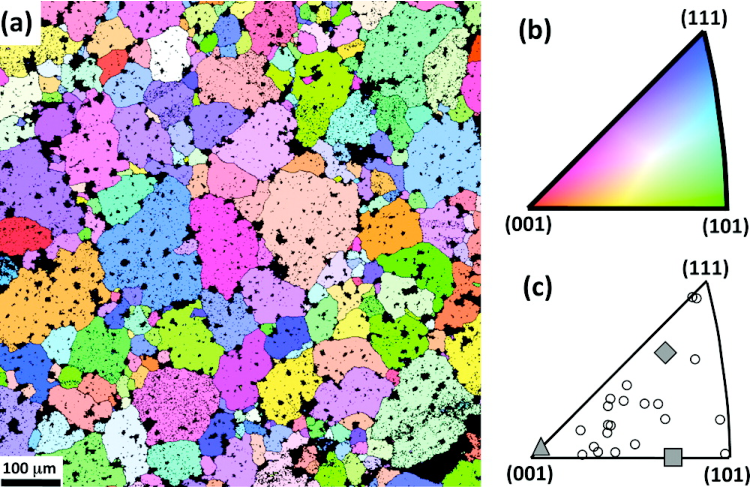
\includegraphics[width=\textwidth]{bfofig1.pdf}
		\caption[Orientation data for examined \ce{BiFeO3} grains]{%
			(a) Inverse pole figure map showing the grain orientations 
			in the area of the polycrystalline \ce{BiFeO3} surface where 
			the surface reactivity was determined. Each color corresponds 
			to an orientation in (b). The orientations of the 24 grains 
			that were studied in detail are illustrated in (c). The grains 
			with orientations marked by the triangle, square, and diamond 
			are discussed in more detail below.}
		\label{fig:bfofig1}
\end{figure}
Each pixel is colored by orientation according to the legend in Figure
\ref{fig:bfofig1}(b). Typically, the undetermined orientations (black points) occur
because there was a grain boundary, pore, or minority phase at that position. The regions
of constant color correspond to grains of constant orientation. Twenty-four of these
grains were selected for closer examination and their orientations are illustrated in
Figure \ref{fig:bfofig1}(c). Each point in Figure \ref{fig:bfofig1}(c) represents an
orientation in the standard stereographic triangle of distinguishable crystal
orientations.

\abbr{AFM} images of the grain with the orientation marked by the triangle in Figure
\ref{fig:bfofig1}(c) are shown in Figure \ref{fig:bfofig2}.
\begin{figure}
	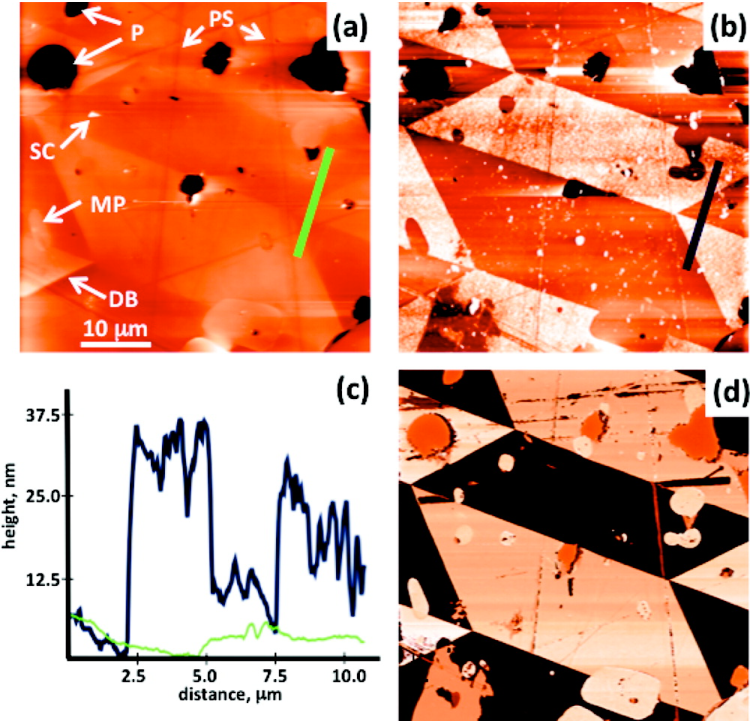
\includegraphics[width=\textwidth]{bfofig2.pdf}
	\caption[Topographic \abbr{AFM} images of \ce{BiFeO3} grain surface]{%
		Topographic \abbr{AFM} images of \ce{BiFeO3} grain surface 
		with a (001) orientation (a) before and (b) after the 
		photochemical reduction of Ag. The topographic contrast 
		in both images is \SI{60}{\nano\meter} from bright to 
		dark. (c) Height profile corresponding to the lines drawn 
		in a and b demonstrating the height of silver deposits 
		and the spatially selective nature of silver deposition. 
		(d) Out-of-plane \abbr{PFM} phase image of the same area of the 
		sample. Dark contrast in the image corresponds to regions 
		with a -180\si{\degree} phase shift (positive polarization) 
		and bright regions correspond to a phase shift of 0\si{\degree} 
		(negative polarization).}
	\label{fig:bfofig2}
\end{figure}
The surface orientation of this grain is, within the experimental uncertainty, (001). The
same location is shown before and after the photochemical reduction of silver in images
(a) and (b) in Figure 2, respectively. Topographic contrast in the \abbr{AFM} images
arises from pores (\abbr{P}), residual polishing scratches (\abbr{PS}), minority phases
(\abbr{MP}), surface contamination \abbr{SC}), and boundaries between ferroelectric
domains (\abbr{DB});\cite{Catalan:2009ca} examples of each feature are labeled on the
micrographs. \label{minorityphase}Regions of minority phase were assigned to round
features within grains in the \abbr{AFM} images. The presence of minority phase in the
bulk was confirmed from the results of X-ray diffraction. These areas are clearly visible
in polarized light optical microscopy and in \abbr{AFM} images. The combination of the
appearance in optical and \abbr{AFM} microscopy and X-ray diffraction results suggests
this assignment as minority phases is appropriate. In Figure \ref{fig:bfofig2}(b), the
reduced silver corresponds to areas of bright contrast in the \abbr{AFM} images. The areas
of silver deposition follow the areas of ferroelectric domains visible on the images of
the clean surface and the heights of the silver deposits vary between 20 and 130 nm.
Height profiles are depicted in Figure \ref{fig:bfofig2}(c) for the lines drawn in the
\abbr{AFM} images shown in images (a) and (b) in Figure \ref{fig:bfofig2} before and after
the reaction. This direct comparison of the same area of the sample shows a clear
distinction in heights for domains before and after the reduction of silver.

After the silver was removed from the sample surface, the sample was returned to the
microscope and the same area was examined using piezoresponse force microscopy
(\abbr{PFM}). The silver was removed by wiping the surface with a cotton swab and rinsing
with deionized water. \abbr{AFM} scans after cleaning show that all silver was removed
from the sample. Figure \ref{fig:bfofig2}(d) shows a \abbr{PFM} phase image for the same
area of the sample surface depicted in images (a) and (b) in Figure \ref{fig:bfofig2}. The
direction of the polarization vector determines the phase lag between the AC bias of the
tip and the deflection. Throughout this chapter, domains with a positive out-of-plane
polarization will be referred to as "positive" domains and domains with a negative
out-of-plane polarization will be referred to as "negative" domains. In the \abbr{PFM}
images, the phase lag is 180\si{\degree} for positive domains and 0\si{\degree} for
negative domains.\cite{Kalinin:2002hq,Kalinin:2006bg,Kalinin:2001jg,Kalinin:2004hu} Areas
of silver deposition correspond to domains that appear dark in the \abbr{PFM} image. These
areas correspond to a phase lag of 180\si{\degree}, consistent with positive domains.
Bright areas in the \abbr{PFM} image, consistent with negative domains, correspond to
areas without significant silver reduction.

The domain polarization is along <111> type directions and the orientations of the
boundaries between domains are {110} and {100} type planes for 71\si{\degree} and
109\si{\degree} domain boundaries, respectively.\cite{Catalan:2009ca} For 180\si{\degree}
boundaries, where the polarization vectors are anti-parallel, the plane can take any
orientation in the zone of [111]. Therefore, in the general case, we can expect to see
both straight and wavy boundaries. When the 71\si{\degree} and 109\si{\degree} domain
boundaries intersect the (001) surface, they create traces that intersect at
45\si{\degree} and 90\si{\degree}. Note that all of the straight lines that appear to be
domain boundaries in Figure \ref{fig:bfofig2} are consistent with these expected angles.
Grains of other orientations consistently showed either straight lines traversing the
entire grain, or combinations of straight and curved boundaries, as illustrated in Figure
\ref{fig:bfofig3}.

Figure \ref{fig:bfofig3} shows \abbr{AFM} topography, \abbr{PFM} phase, and height profile
comparisons for two additional grains of the 24 orientations in Figure
\ref{fig:bfofig1}(c).
\begin{figure}
		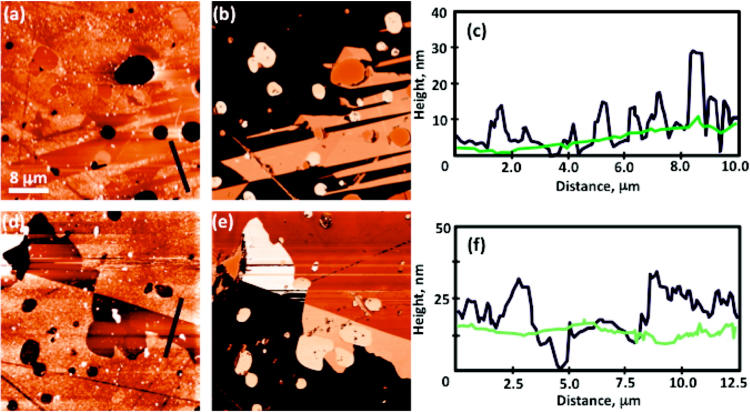
\includegraphics[width=\textwidth]{bfofig3.pdf}
		\caption[Scanning probe data for additional grains]{%
			(a, d) Topographic images of \ce{BiFeO3} grains after the 
			photochemical reduction of silver. Light to dark contrast 
			for both images is \SI{60}{\nano\meter}. (b, e) Out-of-plane 
			\abbr{PFM} phase images for the same areas. Dark contrast corresponds 
			to a positive out of plane polarization. (c, f) Height profiles 
			corresponding to the line drawn in a and d. The green lines 
			show the topography before the reaction.}
		\label{fig:bfofig3}
\end{figure}
The orientation of the grain in Figure \ref{fig:bfofig3}(a) is indicated by the diamond in
Figure \ref{fig:bfofig1}(c) and the orientation of the grain in Figure
\ref{fig:bfofig3}(d) is indicated by the square. These results, and those shown in Figure
\ref{fig:bfofig2}, are representative of all of the orientations. Silver was reduced on
the surface in patterns corresponding to the underlying domain structure. Positive domains
promoted silver reduction and negative domains had little to no solid product on the
surface after reaction. The amounts of silver reduced on the surfaces shown in Figure
\ref{fig:bfofig3} are similar to the amounts in Figure \ref{fig:bfofig2} and are
characteristic of all of the grain orientations in Figure \ref{fig:bfofig1}(c). In other
words, no systematic variation in reactivity could be detected as a function of
orientation in this work. However, later studies of a larger number of grains has shown
some variation in the reactivity as a function of orientation, though the correlation with
domain structure was always observed. In other words, the domain pattern reactivity still
dominates the spatial selectivity, but certain orientations did have increased reactivity
on the locally reactive domains.



To probe the electronic properties of the sample, current-voltage curves were acquired in
the scanning tunneling spectroscopy mode. Because this was done in air, we assume that the
tip is actually in weak contact with the sample. Current-voltage curves were acquired at
periodic positions on the surface and all appeared similar. A typical curve is shown in
Figure \ref{fig:bfofig4},
\begin{figure}
\begin{center}
	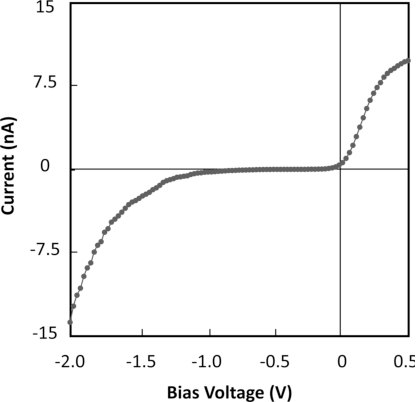
\includegraphics[width=0.5\textwidth]{bfofig4.pdf}
		\caption[Scanning tunneling spectroscopy measurement of \ce{BiFeO3}]{%
			Current versus tip bias measured in a scanning tunneling spectroscopy 
	experiment on the surface of \ce{BiFeO3}.}
	\label{fig:bfofig4}
\end{center}
\end{figure}
%\sidefigure[Scanning tunneling spectroscopy measurement of \ce{BiFeO3}]{%
%	Current versus tip bias measured in a scanning tunneling spectroscopy 
%	experiment on the surface of \ce{BiFeO3}.
%	\label{fig:bfofig4}
%	}{%
%	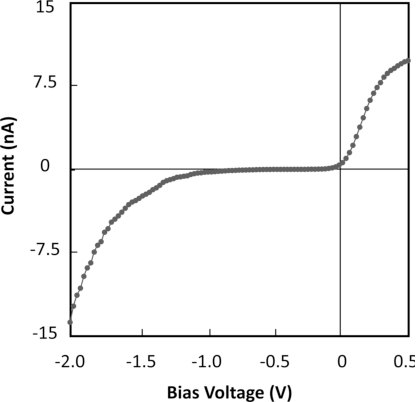
\includegraphics[width=\marginparwidth]{bfofig4.pdf}
%}{-2}
where rectifying behavior is observed; current flows from the sample to the tip at all
positive biases but no current flows from the tip to the sample until the tip is at least
one volt more negative than the sample. This behavior is characteristic of a p-type
semiconductor where the Fermi level is near the lower edge of the band gap. When the tip
is positive with respect to the sample, electrons flow from occupied states in the valence
band to the tip. When the tip is made more negative than the sample, the Fermi level of
the tip moves through the band gap of the sample until it reaches empty states near the
conduction band edge, and electrons can then flow from the tip to the sample. This is
illustrated with schematic energy level diagrams in \figureref{stsdiagram}. A simple
two-point resistivity measurement showed that the sample was only weakly conductive and
had a resistivity of approximately \SI{1e7}{\ohm\centi\meter}.
%\sidefigure[theory of scanning tunneling spectroscopy measurements]{%
%	Diagram showing the theory of scanning tunneling spectroscopy measurements.
%	When the tip is within the band gap, current cannot flow. As the tip is
%	moved to a more positive voltage than the Fermi level, current begins to flow 
%	from the sample to the tip. When the tip is moved to a voltage more negative
%	than the Fermi level, electrons flow from the tip to the sample. The voltage
%	difference between the onsets of current flow is roughly equal to the band gap.
%	The horizontal position of the curve determines the carrier type.
%	\label{fig:stsdiagram}
%	}{%
%	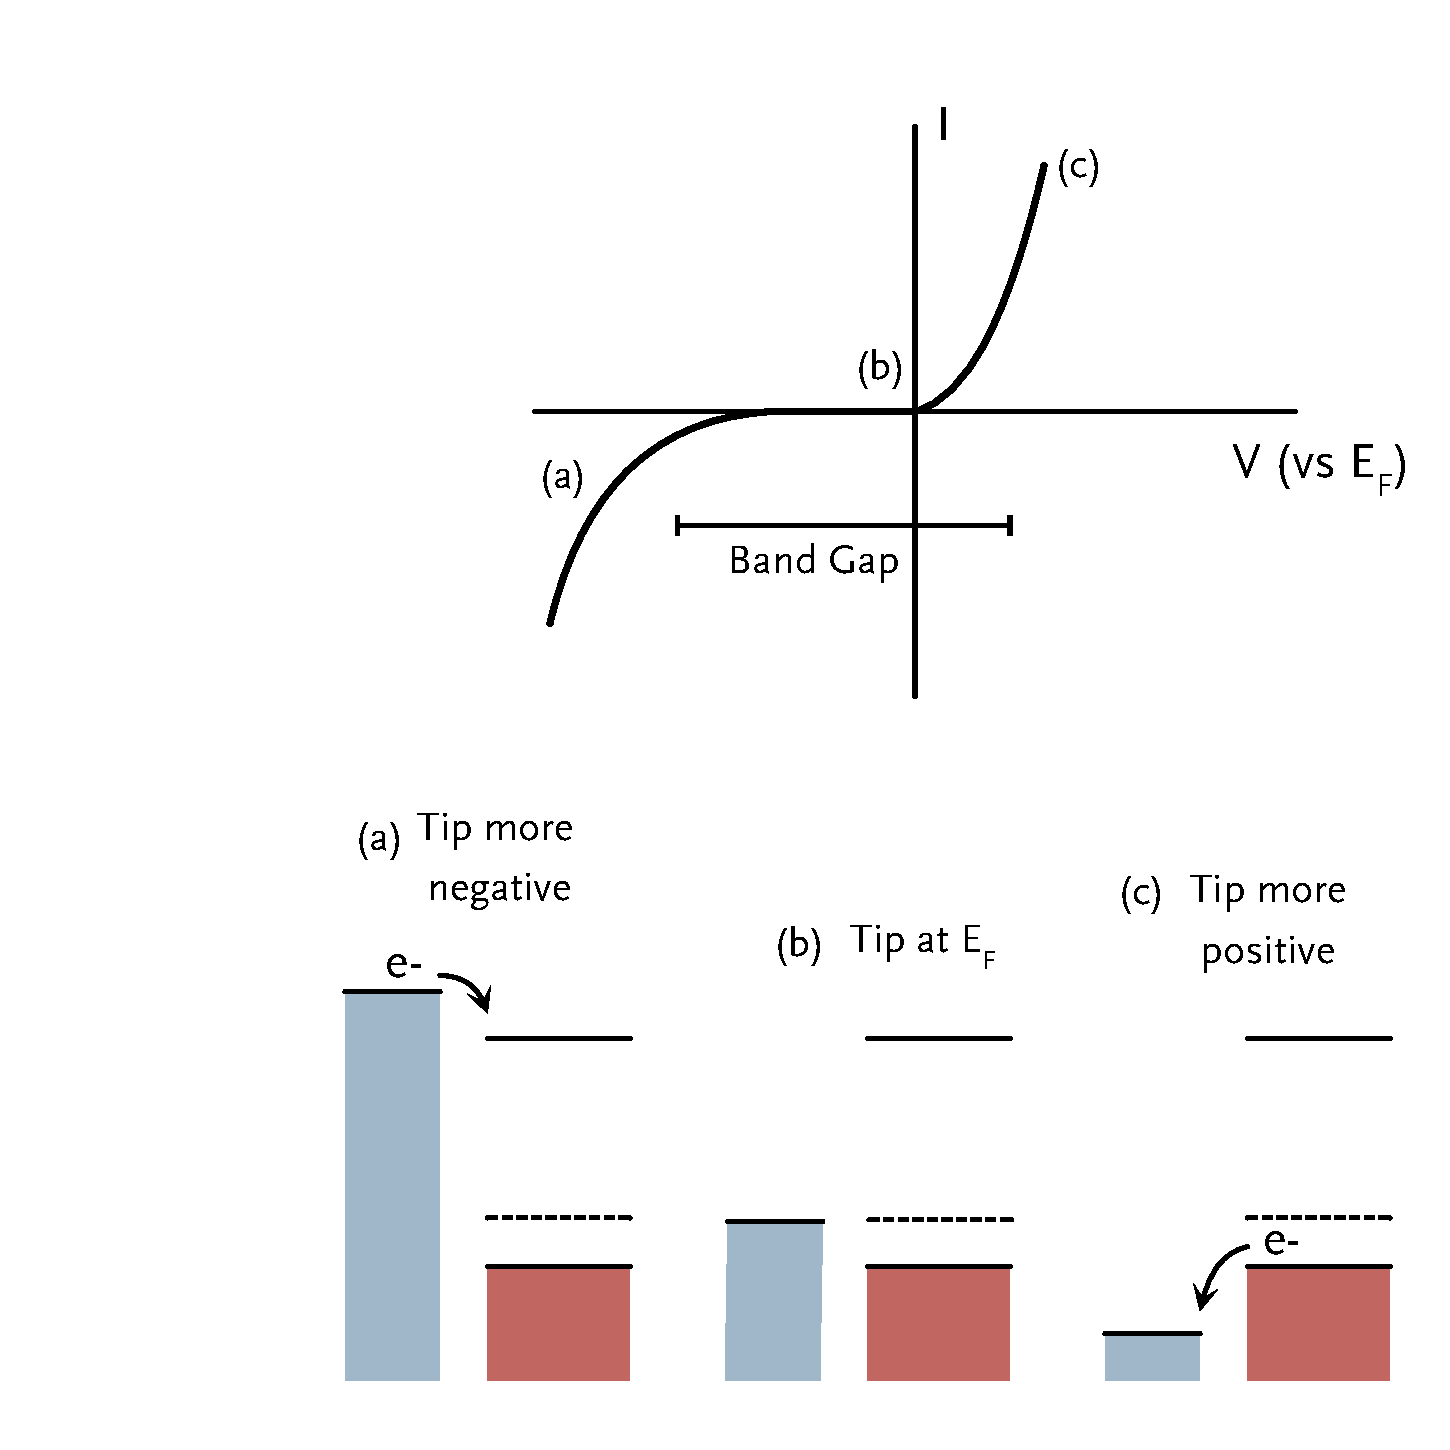
\includegraphics[width=\marginparwidth]{stsdiagram.pdf}
%}{0} %
\begin{figure}
	\centerline{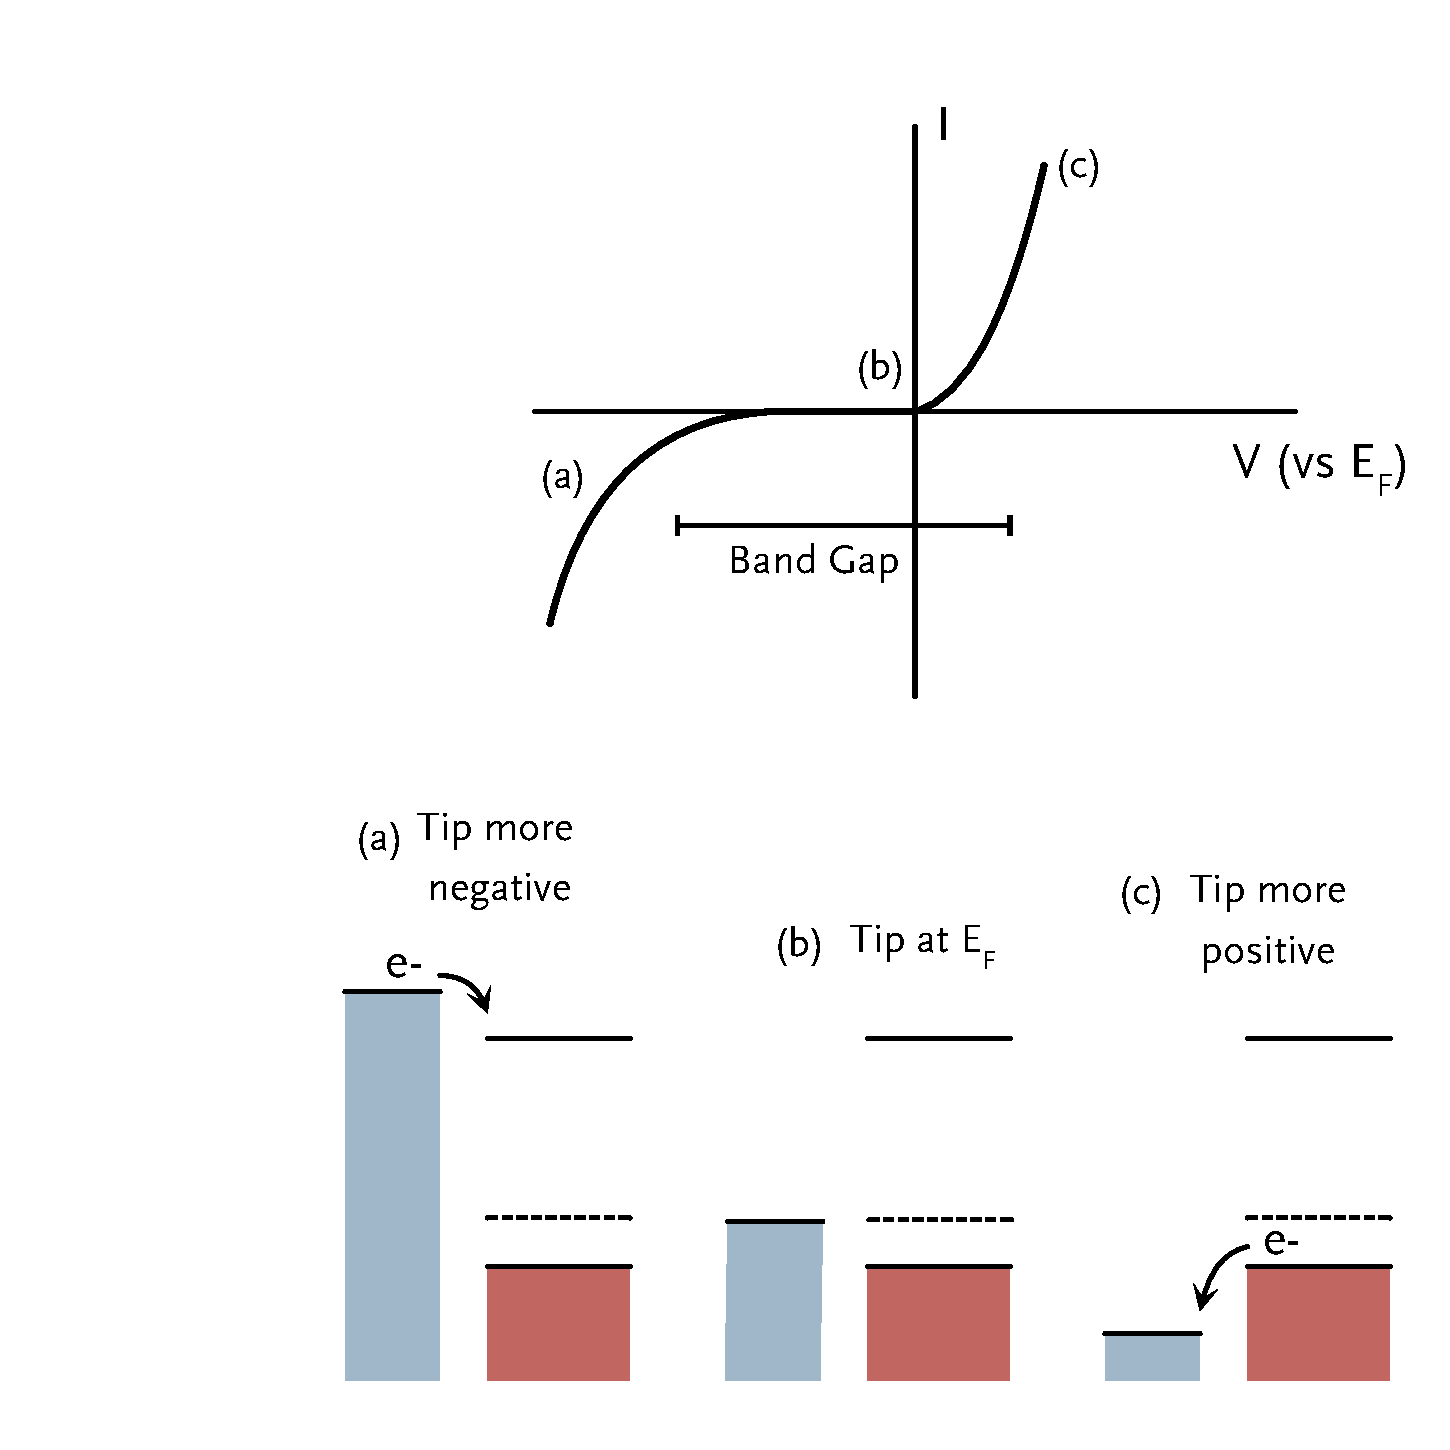
\includegraphics[width=0.6\textwidth]{stsdiagram.pdf}}
		\caption[Theory of scanning tunneling spectroscopy measurements]{%
			Diagram showing the theory of scanning tunneling spectroscopy 
			measurements. When the tip is within the band gap, current cannot
			 flow. As the tip is moved to a more positive voltage than the 
			 Fermi level, current begins to flow from the sample to the tip. 
			 When the tip is moved to a voltage more negative than the Fermi 
			 level, electrons flow from the tip to the sample. The voltage 
			 difference between the onsets of current flow is roughly equal 
			 to the band gap. The horizontal position of the curve determines 
			 the carrier type.}
	\label{fig:stsdiagram}
\end{figure}

\section{Discussion}\label{sec:ch7discussion}

The results presented here indicate that the photochemical reduction of silver, initiated
by visible light, is spatially selective on the \ce{BiFeO3} surface. This is similar to
what has been observed previously on \ce{BaTiO3}, \ce{SrTiO3}, and \abbr{PZT} when
illuminated under \abbr{UV}
light.\cite{Burbure:2010go,Giocondi:2001bi,Giocondi:2003wc,Lowekamp:1998ks,Dunn:2007ja}
Here we propose a model for the surface electronic band structure of \ce{BiFeO3}, and how
it is affected by ferroelectric polarization, to explain the observed reactivity. The
proposed energy level structure, shown in Figure \ref{fig:bfofig5}, is based upon a number
of assumptions. First, the electron affinity of the \ce{BiFeO3} (\SI{4.6}{\electronvolt})
was approximated using the method described by Morrison.\cite{Morrison:1980va} The band
gap of \ce{BiFeO3} has been reported over a wide range (2.2-\SI{2.7}{\electronvolt}) in
different sources;\cite{Basu:2008hd,Choi:2009gh,Gao:2006fg} in the construction of Figure
\ref{fig:bfofig5}, we assumed a band gap of \SI{2.5}{\electronvolt}. Most reports in the
literature indicate that \ce{BiFeO3} is p-type\cite{Vengalis:2008vi,Yang:2008fo} and this
is consistent with the current-voltage response shown in Figure~\ref{fig:bfofig4}.
\begin{figure}[htbp]
\begin{center}
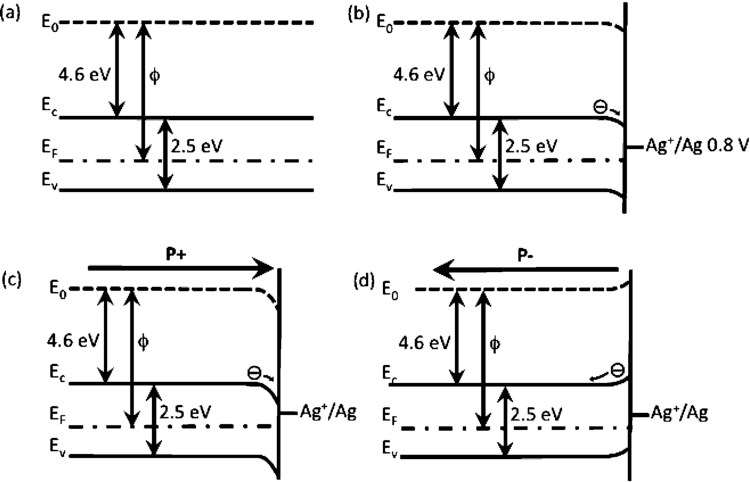
\includegraphics[width=\textwidth]{bfofig5.pdf}
\caption[Schematic band diagrams for \ce{BiFeO3}]{Schematic band diagrams for \ce{BiFeO3}.
In the figure,  is the work function, E$_0$, E$_c$, E$_F$, and E$_v$ are the energy levels
of a free electron, the conduction band edge, the Fermi level, and the valence band edge,
respectively. (a) Bands in bulk \ce{BiFeO3}. (b) Bands of \ce{BiFeO3} in contact with
solution, with the standard redox potential for \ce{Ag+}/Ag labeled vs the normal hydrogen
electrode. (c) Bands in contact with solution and a positive out-of-plane polarization.
(d) Bands in contact with solution and a negative out-of-plane polarization.}
\label{fig:bfofig5}
\end{center}
\end{figure}

Figures \ref{fig:bfofig5}(a) and \ref{fig:bfofig5}(b) compare the band positions in bulk
\ce{BiFeO3} with those near the surface when in contact with solution, with no
out-of-plane polarization. Interface states cause downward band bending at the surface of
a p-type semiconductor in contact with water.\cite{Morrison:1980va} In this case,
electron-hole pairs generated within the depletion region are driven apart by the electric
field. Electrons are driven towards the surface and holes are driven away from the
surface. When electrons reach the surface, they can reduce adsorbed species. Panels (c)
and (d) in Figure \ref{fig:bfofig5} show the effect of ferroelectric polarization on the
band bending near the surface. The polarization vector in positive domains, depicted in
Figure \ref{fig:bfofig5}(c), causes an increased accumulation of negative charge just
below the surface. Band edge energies are driven further downward and the driving force
for electrons to reach the surface and participate in photochemical reduction is
increased. The opposite is true for a negative domain, which is depicted in Figure
\ref{fig:bfofig5}(d). The negative out-of-plane component of polarization causes an
increase in positive charge just below the surface and this reduces the downward band
bending. If the magnitude of the polarization vector is large enough, the bands bend
upwards. We take the experimental observation that silver does not reduce on the surfaces
of negative domains as evidence that the bands are bent upward and depict them as such in
Figure \ref{fig:bfofig5}(d), creating a barrier for electrons. In other words,
photogenerated electrons within the band bending region are driven away from the surface
and this shuts off the silver reduction reaction in these domains. Because electrons and
holes are driven to different areas of the surface, the chances of charge carrier
recombination are reduced. Additionally, intermediate species produced during the reaction
are located in physically separate areas of the surface, reducing back reaction. Because
of this, the fields generated by the ferroelectric polarization might improve the
efficiency of photochemical reactions. Finally, we note that throughout this discussion,
we have ignored the effect of adsorption from the solution. In this case, we would expect
aqueous \ce{Ag+} cations to enrich or adsorb at the surfaces of negative domains and be
repelled from positive domains. Because reduced silver is found only on the positive
domains, the observed spatially selective reactivity is not consistent with adsorption
processes.

There are two proposed mechanisms for the orientation dependence of the reactivity of a
ferroelectric material. The first is that photochemical reactions on metal oxides are
anisotropic.\cite{Giocondi:2003wc,Lowekamp:1998ks,MorrisHotsenpiller:1998jq,Ohno:2002fn,
Taguchi:2003hs} While the origins of this anisotropy have not been clearly established,
they are presumably connected to the orientation dependence of surface structure,
composition, and the exact positions of band edges on the surface.
\cite{Giocondi:2003wc,Giocondi:2007fa} This phenomenon is potentially important in the
design of a photolysis catalyst.\cite{Sosnowchik:2010jr}

The second mechanism by which crystal orientation might affect reactivity relates to the
crystallographic restrictions on domain polarization. For a given ferroelectric material,
the direction of ferroelectric polarization is limited to a distinct set of crystal
directions. In the case of \ce{BiFeO3}, the polarization occurs along the 111 family of
directions.\cite{Anonymous:2011wx} The out-of-plane component of the polarization vector
is thought to play the most significant role in affecting photochemical activity. Varying
the grain orientation changes the possible values of the out-of-plane component of each of
the possible polarization directions. For example, a (111)-oriented crystal can have two
antiparallel polarization vectors pointing perpendicular to the surface. The remaining six
directions point 29\si{\degree} above or below the surface plane, greatly reducing the out
of plane component of polarization. In the case of a (001)-oriented grain, all of the
polarization vectors point 54\si{\degree} above or below the surface, resulting in an
equal out-of-plane magnitude of polarization for all directions. Dunn and
co-workers\cite{Dunn:2007cx} reported on differences in the photochemical reduction of Ag
on (001) and (111) oriented \abbr{PZT}, finding that that positive domains in films of
both orientations have a similar reactivity, but that negative domains completely stop the
reactivity only on the (111) orientation where the polarization is perpendicular to the
surface. Burbure and co-workers(10) reported on the relative reactivity of (001), (011),
and (111) \ce{BaTiO3} (which is polarized along [100]), and found comparable activity for
reduction on all three surfaces.

In the current study, spatially selective reactivity was observed for all grain
orientations. Contrary to the observations on \abbr{PZT} thin films, even grains with the
(001) orientation strongly suppress the reduction of silver in the negative domains (see
Figure \ref{fig:bfofig2}). This difference cannot be explained by differences in the
polarization: \abbr{PZT} is reported to have a larger remnant polarization than
\ce{BiFeO3} and that would favor increased spatial selectivity in \abbr{PZT}, counter to
what is observed.\cite{Kobayashi:2005wx} It is possible that differences in the
microstructure might account for differences in the reactivity. The \ce{BiFeO3} crystals
studied here were many tens of micrometers in extent, while the \abbr{PZT} was a
\SI{70}{\nano\meter} thick film with grains of similar sizes.\cite{Dunn:2007cx} Because
there are geometric constraints on the development of space charges in nano-sized grains,
it is possible that the band bending regions are larger in the microcrystalline
\ce{BiFeO3} samples studied here.\cite{ALBERY:1984tu}

While the differences between \ce{BiFeO3} and \abbr{PZT} cannot be resolved from the
present observations, the results presented here demonstrate that the ferroelectric domain
structure is more important than grain orientation in determining surface reactivity. In
grains where ferroelectric domains are present, reactivity was observed to be selective
and the heights of reduced silver on the reactive domains did not systematically depend on
grain orientation. This lack of a strong anisotropy in reactivity indicates that the
relative orientation of the polarization vector is sufficient in \ce{BiFeO3} to control
the spatial selectivity, consistent with previously published results for
\ce{BaTiO3}.\cite{Burbure:2010tt} If the relative magnitude of the polarization normal to
the surface determined local reactivity, then (111) oriented \ce{BiFeO3} grains should
have the greatest reactivity in domains with a positive polarization points toward the
outer surface. However, the reactive domains on grains oriented near (111) were not
noticeably more reactive than reactive domains on grains with different orientations. The
same is true for the unreactive, negative domains, where the bands bend upward. A possible
explanation for this behavior is found by comparing the depletion layer width and the
penetration depth of the illumination. If the photon penetration depth is smaller than the
space charge region that results from the ferroelectric polarization, increasing the width
of the space charge layer causes no increase in reactivity. All photogenerated charge
carriers are already created within the space charge region and driven to or from the
surface. Yang et al.\cite{Yang:2009hl} estimate a depletion layer width of
\SI{300}{\nano\meter} for \ce{BiFeO3}. The penetration depth for 460 nm light in
\ce{BiFeO3} is approximately \SI{36}{\nano\meter}, using the extinction coefficient data
from Kumar et al. \cite{Kumar:2008fr} In this case, the space charge region is much larger
than the penetration depth, and any increase in the width of the space charge region will
not increase the photochemical reactivity of the material. As a result, in any domains
where the bands are bend downward, silver is reduced, and in any domains where they are
bent upward, no silver is reduced.

It has recently been shown that thin titania films supported by \ce{BiFeO3} are also
active for silver reduction using the same light source.\cite{Zhang:2011cj} This indicates
that it should be possible to create a heterostructured core-shell photocatalyst of
\ce{BiFeO3} particles coated by a thin layer of titania that will combine the favorable
band edge positions and stability of the titania surface with the light absorbing and
charge separating characteristics of the \ce{BiFeO3} core. The present results suggest
that in such a composite material, the shape of the \ce{BiFeO3} crystals will not be
important, but the size will. To effectively absorb light, the cores will have to be at
least twice the absorption depth and to effectively separate charge, they should be large
enough to sustain a ferroelectric polarization that promotes band bending, and this is
twice the width of the space charge region. Because these two lengths will not generally
be the same, the reactivity may be size dependent.

\section{Conclusion}\label{sec:ch7conclusion}

\ce{BiFeO3} surfaces exhibit spatially selective visible-light photochemical activity.
Silver ions in solution were photochemically reduced by the \ce{BiFeO3}, depositing solid
silver on the surface in patterns corresponding to positive ferroelectric domains. Upward
band bending in the negative domains prevents electrons from reaching the surface and
these locations do not reduce silver. Electric fields arising from ferroelectric domains
at the surface overwhelm anisotropy in the photochemical activity that might arise from
grain orientation alone.